\section{Introduction}

% \begin{itemize}
%     \item Generalization of models is important, and believe that part of what large pretrained LMs bring after seeing lots of texts is generalization
%     \item We talk about two kinds of generalization, lexical, and syntactic
%     \item we focus on the task of knowledge base completion, specifically the probing of LMs for factual information such as barak obama was born in hawaii
%     \item we show that current lms indeed generalize in terms of (simple) language variety, which is surprising
%     \item in order to show that, we create a large graph, with entailment relations, that express some information, with lexical, syntactical and both differences
%     \item we query wikipedia with all the patterns we found, to look for evidencial apparence, to see if these patterns appeared, and extend the graph with additional information about occurrences of the patterns in wikipedia.
%     \item we analyze popular lms and show that in fact, they do not generalize to patterns that did not appear in the training corpus, calling for improved models in the future. 
% \end{itemize}


Pre-trained Language Models (PLMs) have took the NLP field by storm in recents years \cite{elmo,bert,roberta}. Many models used in the field use some kind of PLM, combined with a specific task fine-tuning.
The reason for their success is still unknown, but it is thought that the large amounts of training data allows them to better generalize.

Generalization in NLP is still not well defined, but some clear generalizations are syntactic and lexical. For example, RTE \cite{rte} focused on these kinda of generalization, and created a dataset for testing models ability on this kind of problems.

In this work, we focus on the task of factual knowledge completion \ye{is this the task's name?} and test whether popular PLMs generalize to the actual relation. We find that these models do not generalize to new linguistic patterns with equivalent meaning, but rather succeed in predicting the correct object mainly when the same linguistic utterance appeared in its training data.

In order to test this, we build a large entailment relation graph, which we call \resource{} that contain different ways to describe a relation. \resource{} is a directed graph, which contains edges between patterns with an entailment connection. For example, ``[X] was premiered on [Y]'' entails ``[X] was aired on [Y]'', but not the other way around.

Then, we use spike \cite{spike}, in order to query wikipedia, the main source of factual knowledge of BERT, and part of the factual knowledge of other models, in order to find instances that appeared in these models training data.

Combining \resource{} and the facts that appeared exactly in wikipedia, we can now test the generalization hypothesis, and find that indeed, current PLMs do not generalize to relations that did not appear in wikipedia.
We conduct these experiment on LAMA \cite{lama} that contain 41 different relations, and provide detailed analysis on when these models succeed or fail.

We release this new resource as well as the analysis code to allow future work to repeat these experiments, and track the progress of generalization of PLMs.

\begin{figure}[t!]
\centering

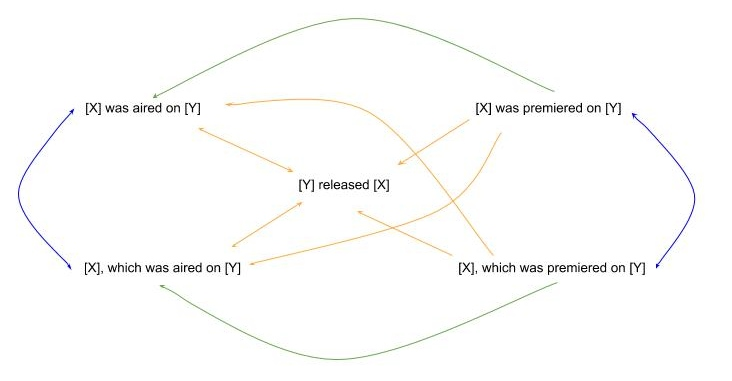
\includegraphics[width=1.\columnwidth]{figures/memorization-entailment-graph-croped}

\caption{(currently ugly, in progress) schematic description of \resource{}. The green, blue and orange arrows stand for syntactic, lexical and both syntactic and lexical transformation. Note that the arrows have a direction, which stand for the entailment direction.}
\label{fig:graph}
\end{figure}